\newpage
\section{Anhang}

\subsection{Anforderungsliste}\label{anforderungliste}

Die erste Version der Anforderungsliste ist nachfolgend angehängt.

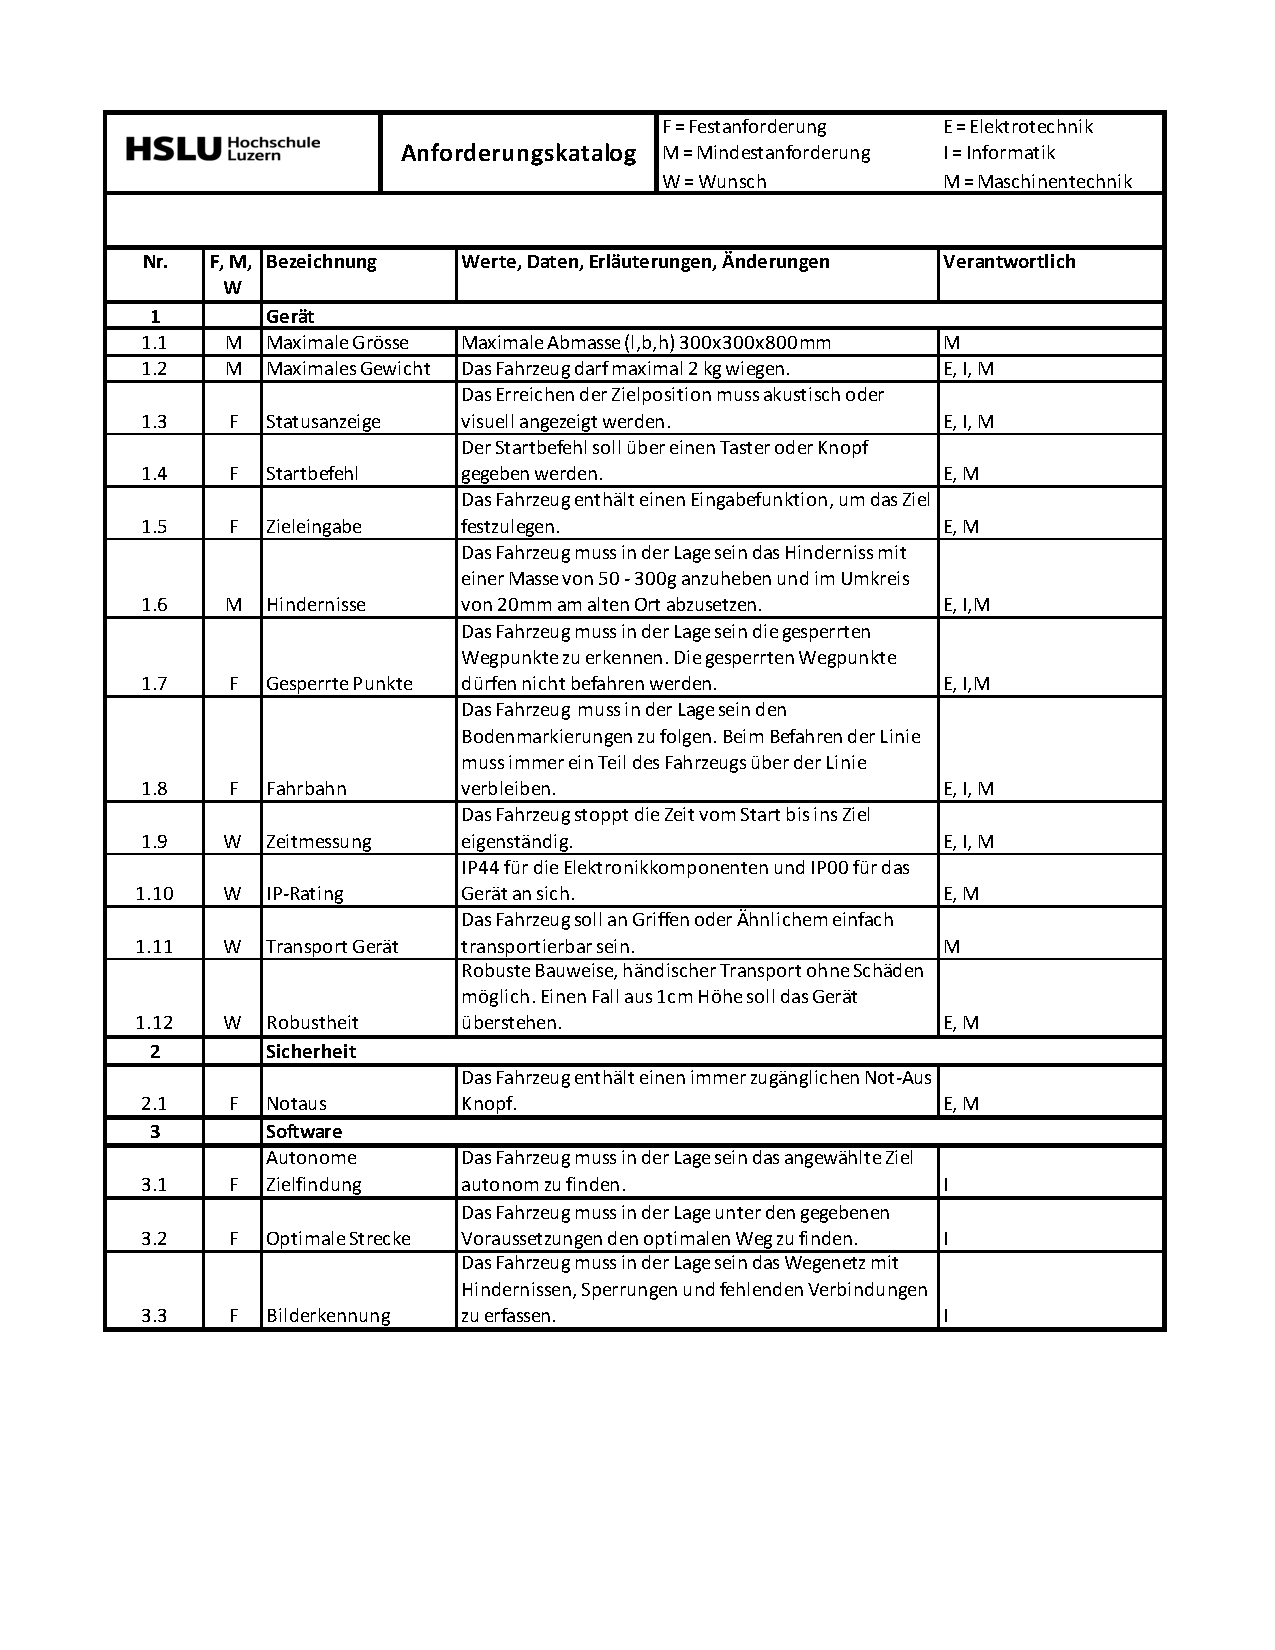
\includepdf[pages=-]{assets/Anforderungsliste_V1.01.pdf}



\begin{landscape}
\subsection{Kommunikationsplan}\label{kommunikationsplan}
Die Kommunikationskanäle sind folgendermassen definiert:

\begin{table}[h]
\centering
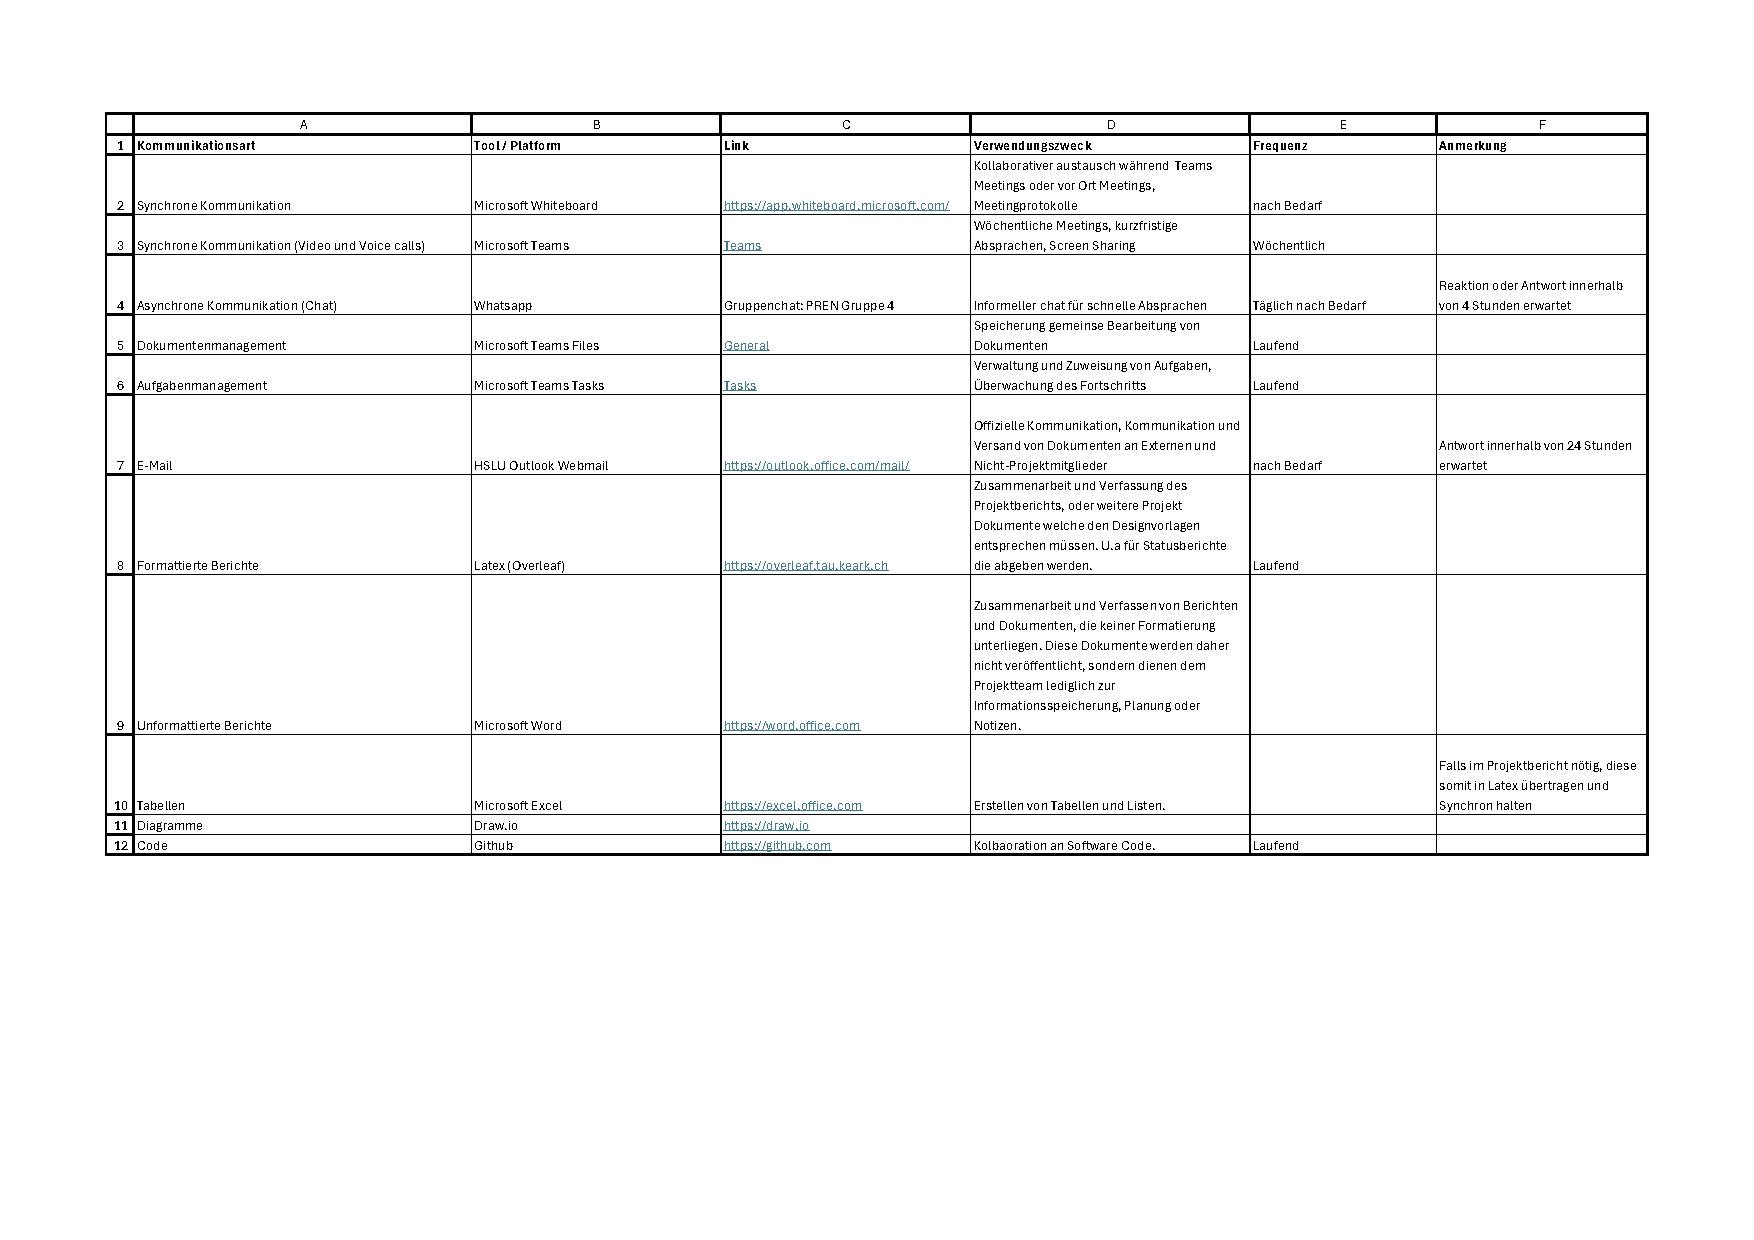
\includegraphics[width=230mm]{assets/Kommunikationschnittstellen.pdf}
\caption{Kommunikationsplan}
\label{table:communications-plan}
\end{table}
\end{landscape}
\newpage


\subsection{Morphologischer Kasten}\label{Morphologischer Kasten}
Nachfolgend die Morphologischen Kästen, unterteilt in die jeweiligen Studiengänge, Elektrotechnik, Informatik und Maschinentechnik.


\begin{table}
\centering
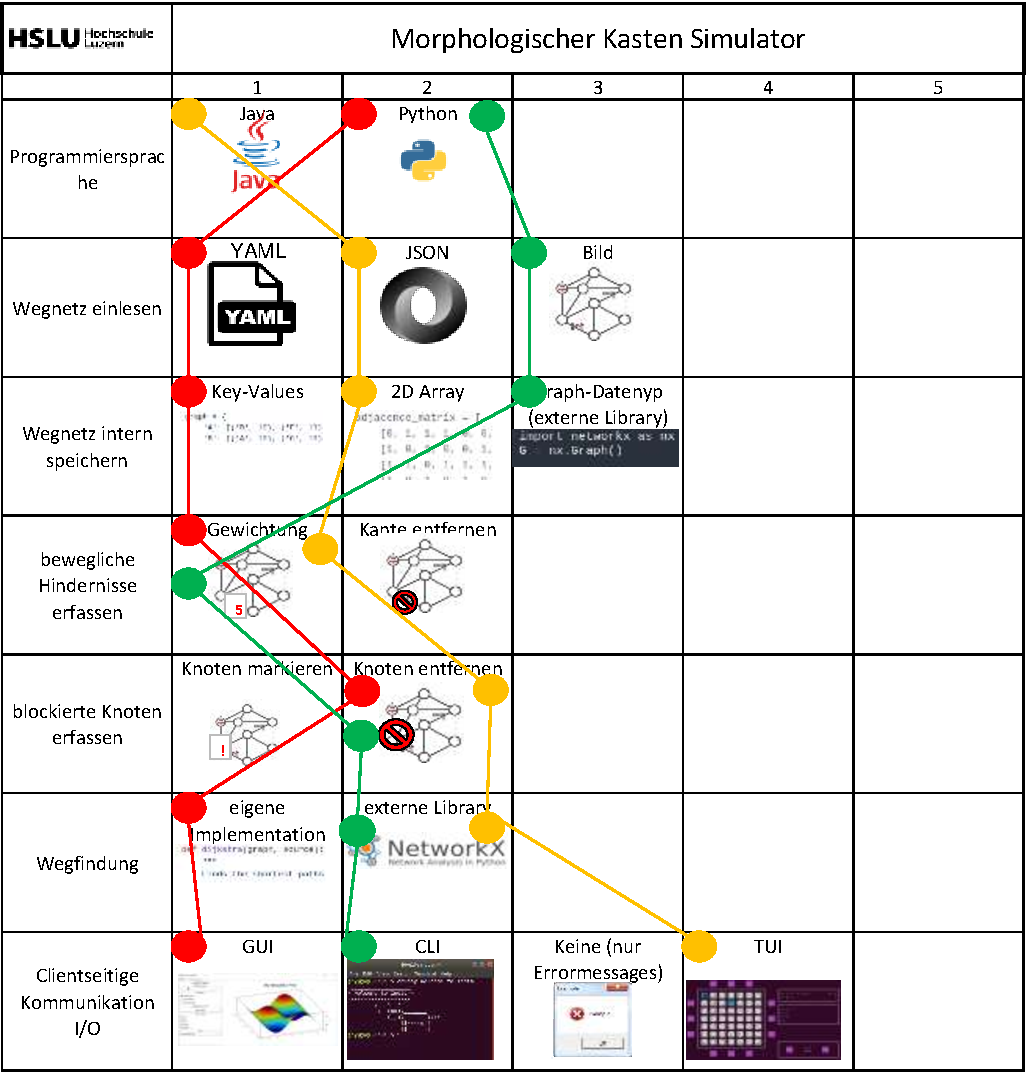
\includegraphics[width=\textwidth]{assets/MK_Simulator.pdf}
\caption{Morphologischer Kasten: Simulator}
\label{table:MK-Simulator}
\end{table}
\newpage


\subsection{Originale Aufgabenstellung}\label{aufgabenstellung}

Nachfolgend ist die originale Aufgabenstellung angehängt.

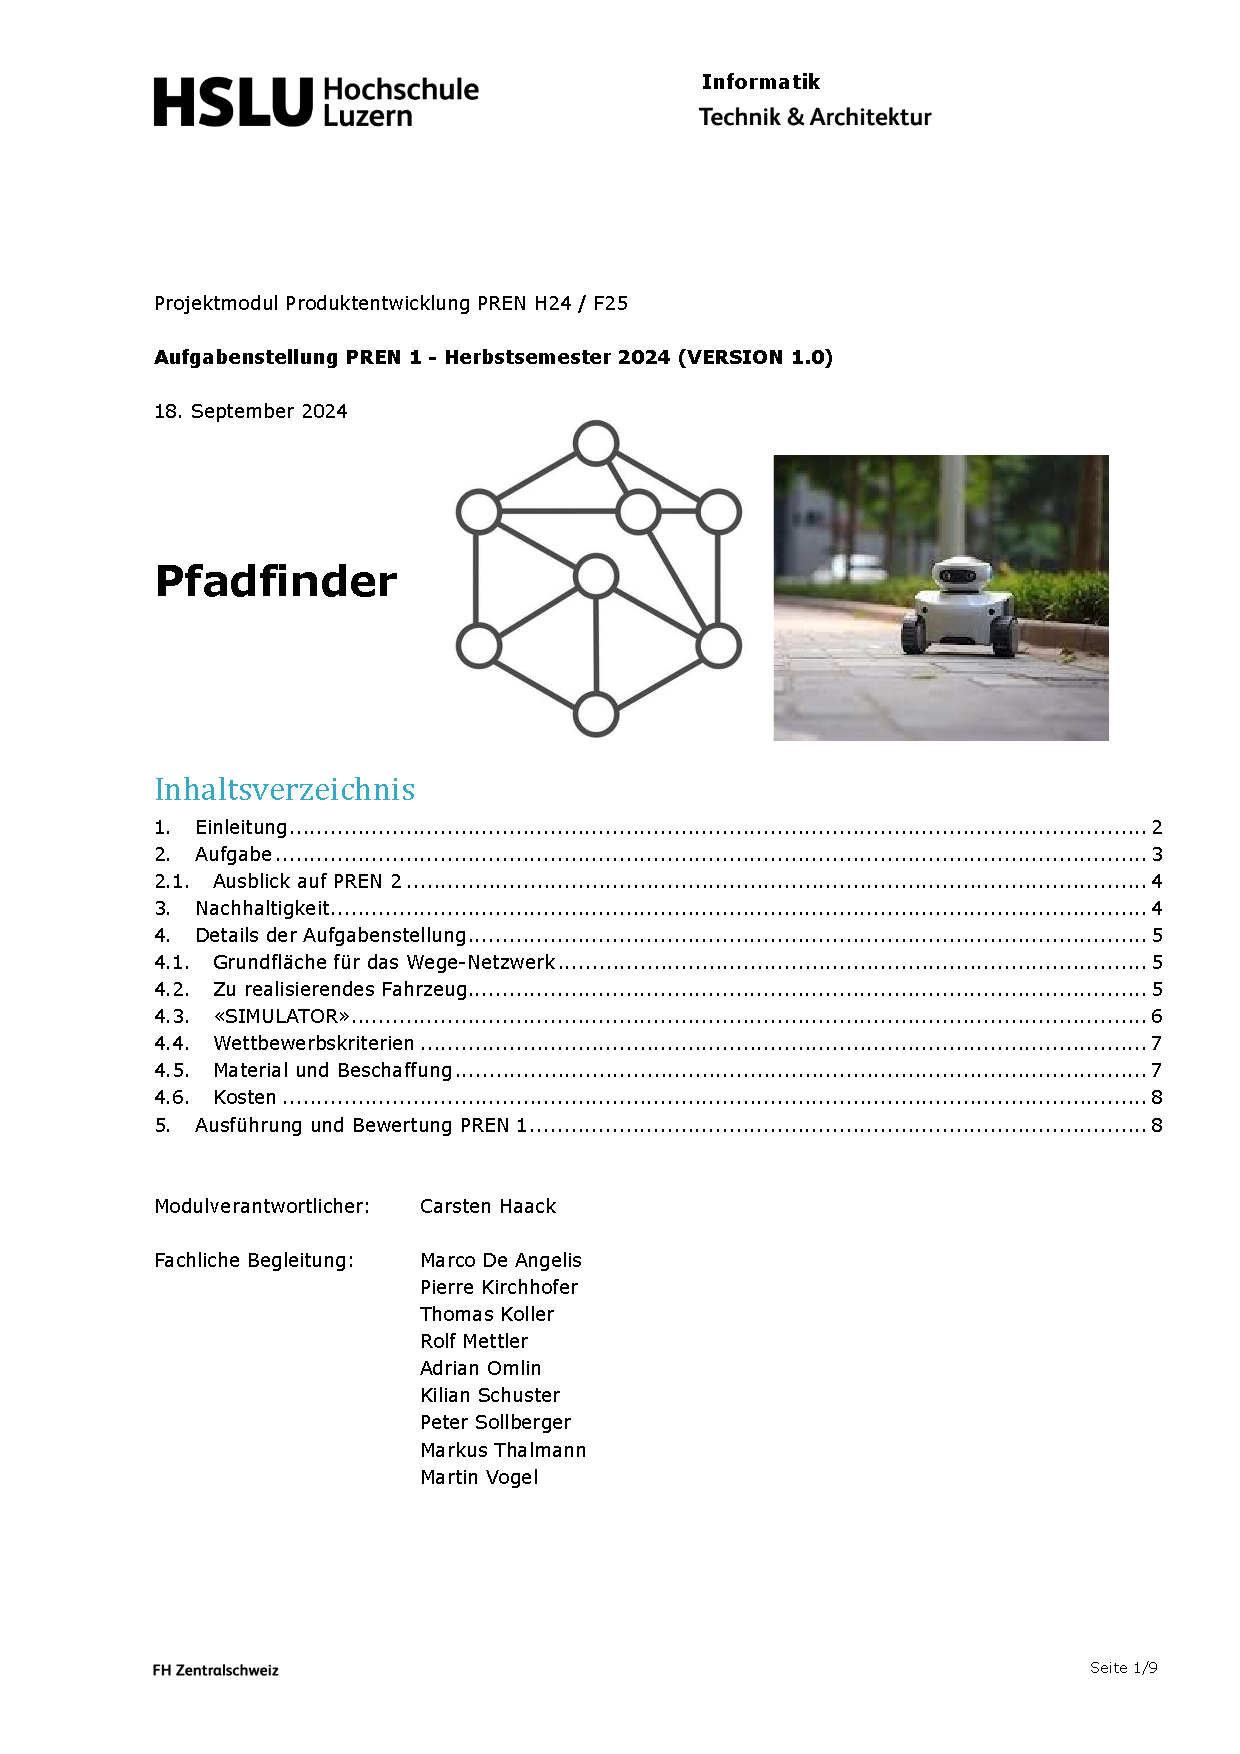
\includepdf[pages=-]{assets/AufgabenstellungPREN1HS24.pdf}
